\chapter{Reverberation Mapping Analysis of NGC4593}

\section{Line Determination}



\begin{figure}[!htbp]
	\centering
	\makebox[\textwidth][c]{%
		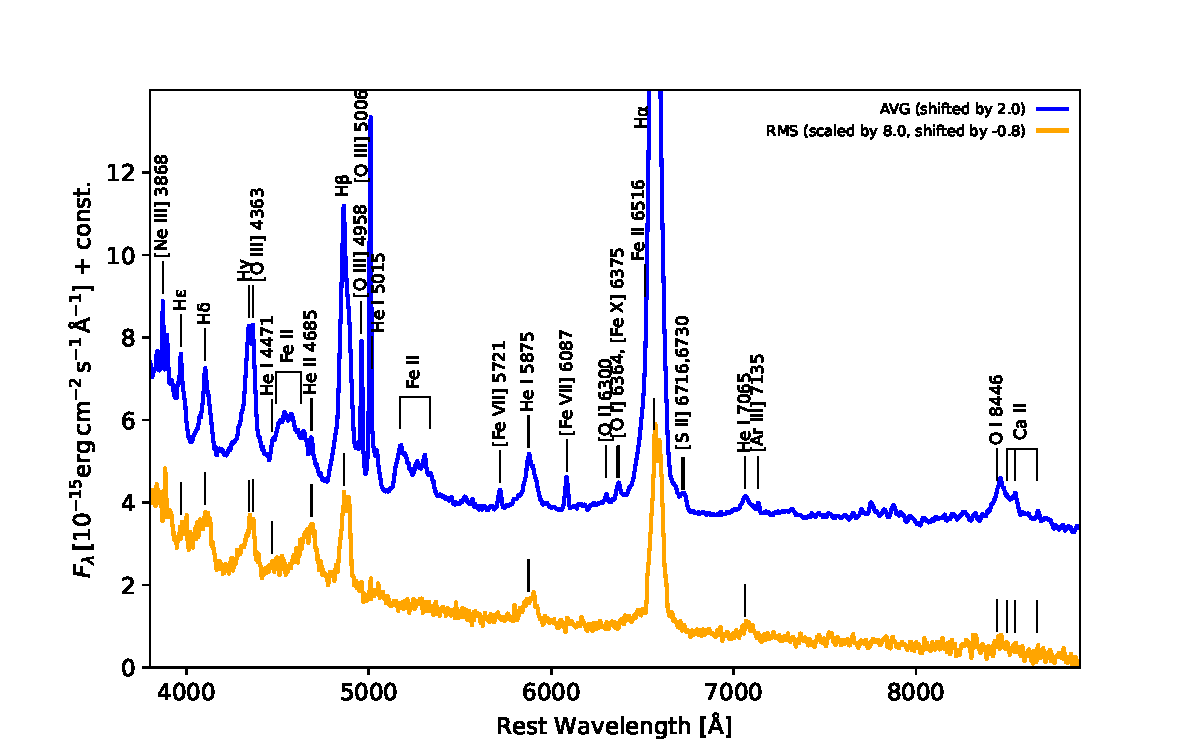
\includegraphics[width=1.2\textwidth]{pictures/Chapter4/avg_rms_spec/avg_rms_spec.pdf}}
	\caption{AVG RMS spectrum}
	\label{fig:AVG_RMS_SPECTRUM}
\end{figure}


\section{Lightcurves}
...
\subsection{Continua}
...
\begin{figure}[!ht]
	\centering
	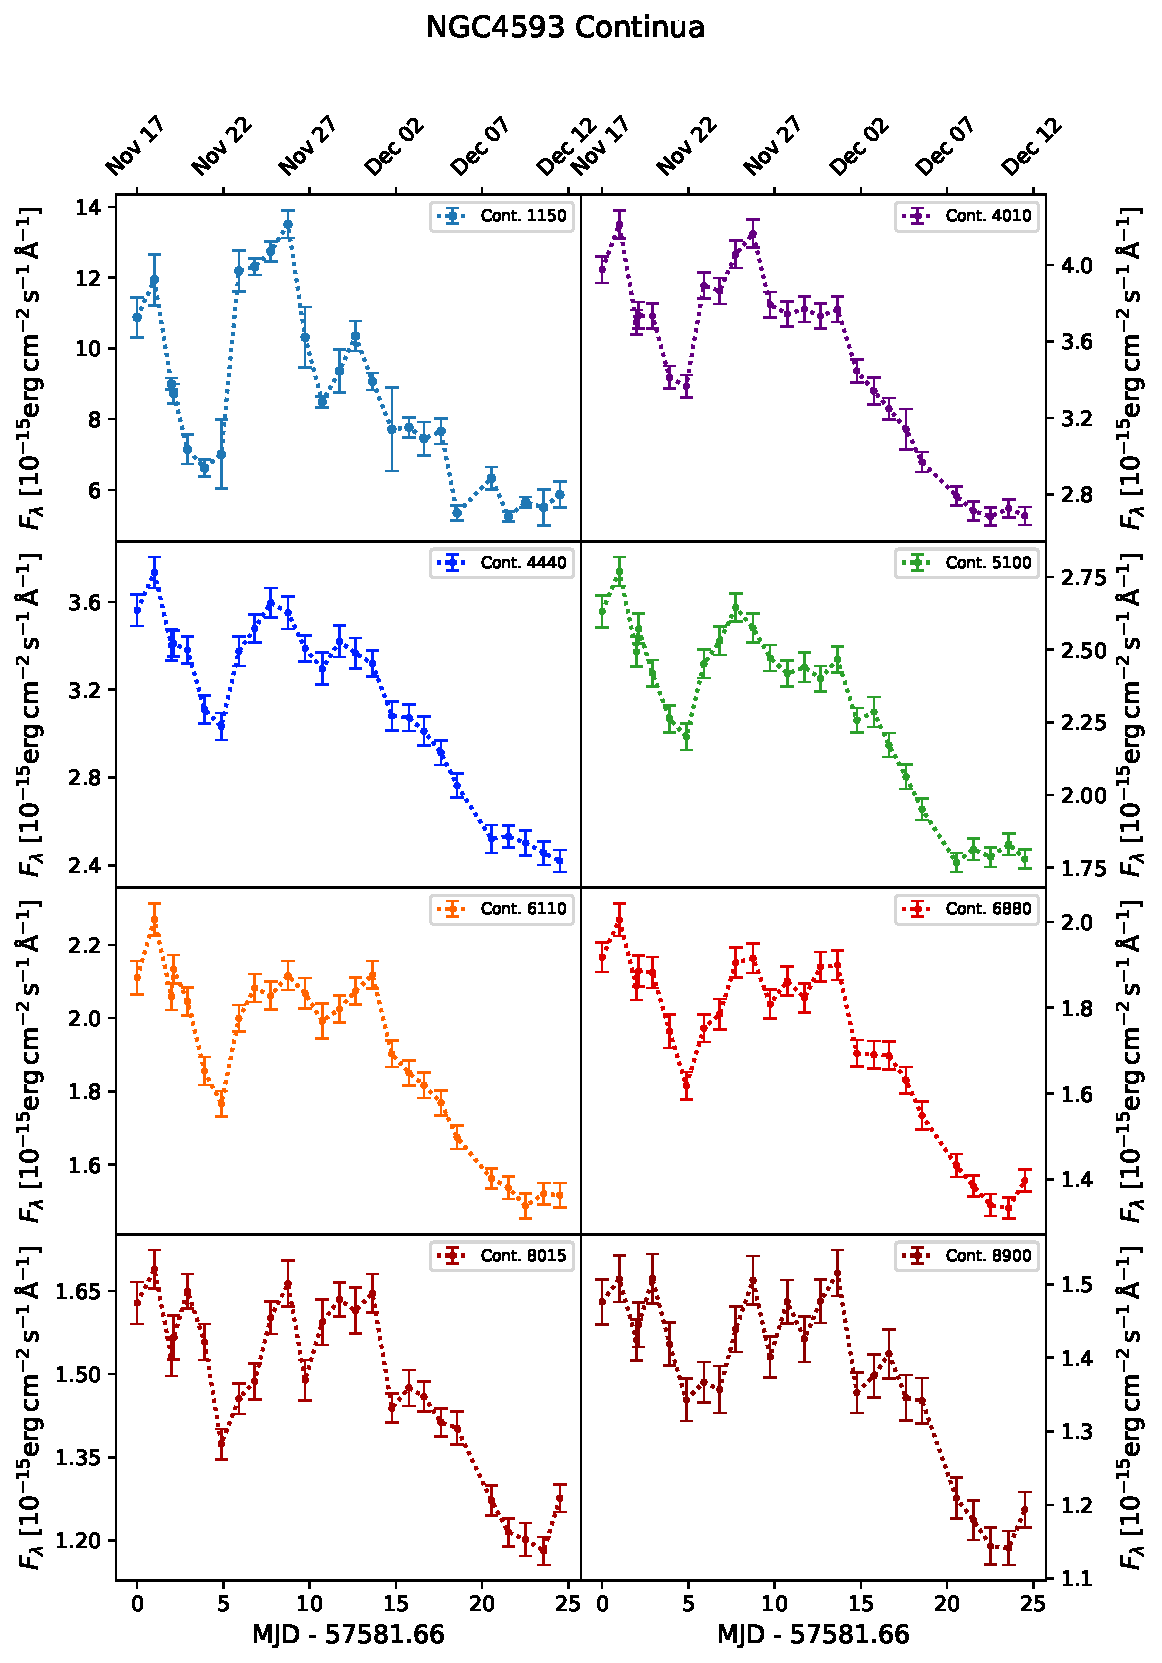
\includegraphics[width=0.9\textwidth]{pictures/Chapter4/lightcurves/NGC4593_Continua.pdf}
	\caption{AVG RMS Spektrum}
	\label{fig:continua_lightcurves}
\end{figure}

\subsection{Emission Lines}
...
\begin{figure}[!ht]
	\centering
	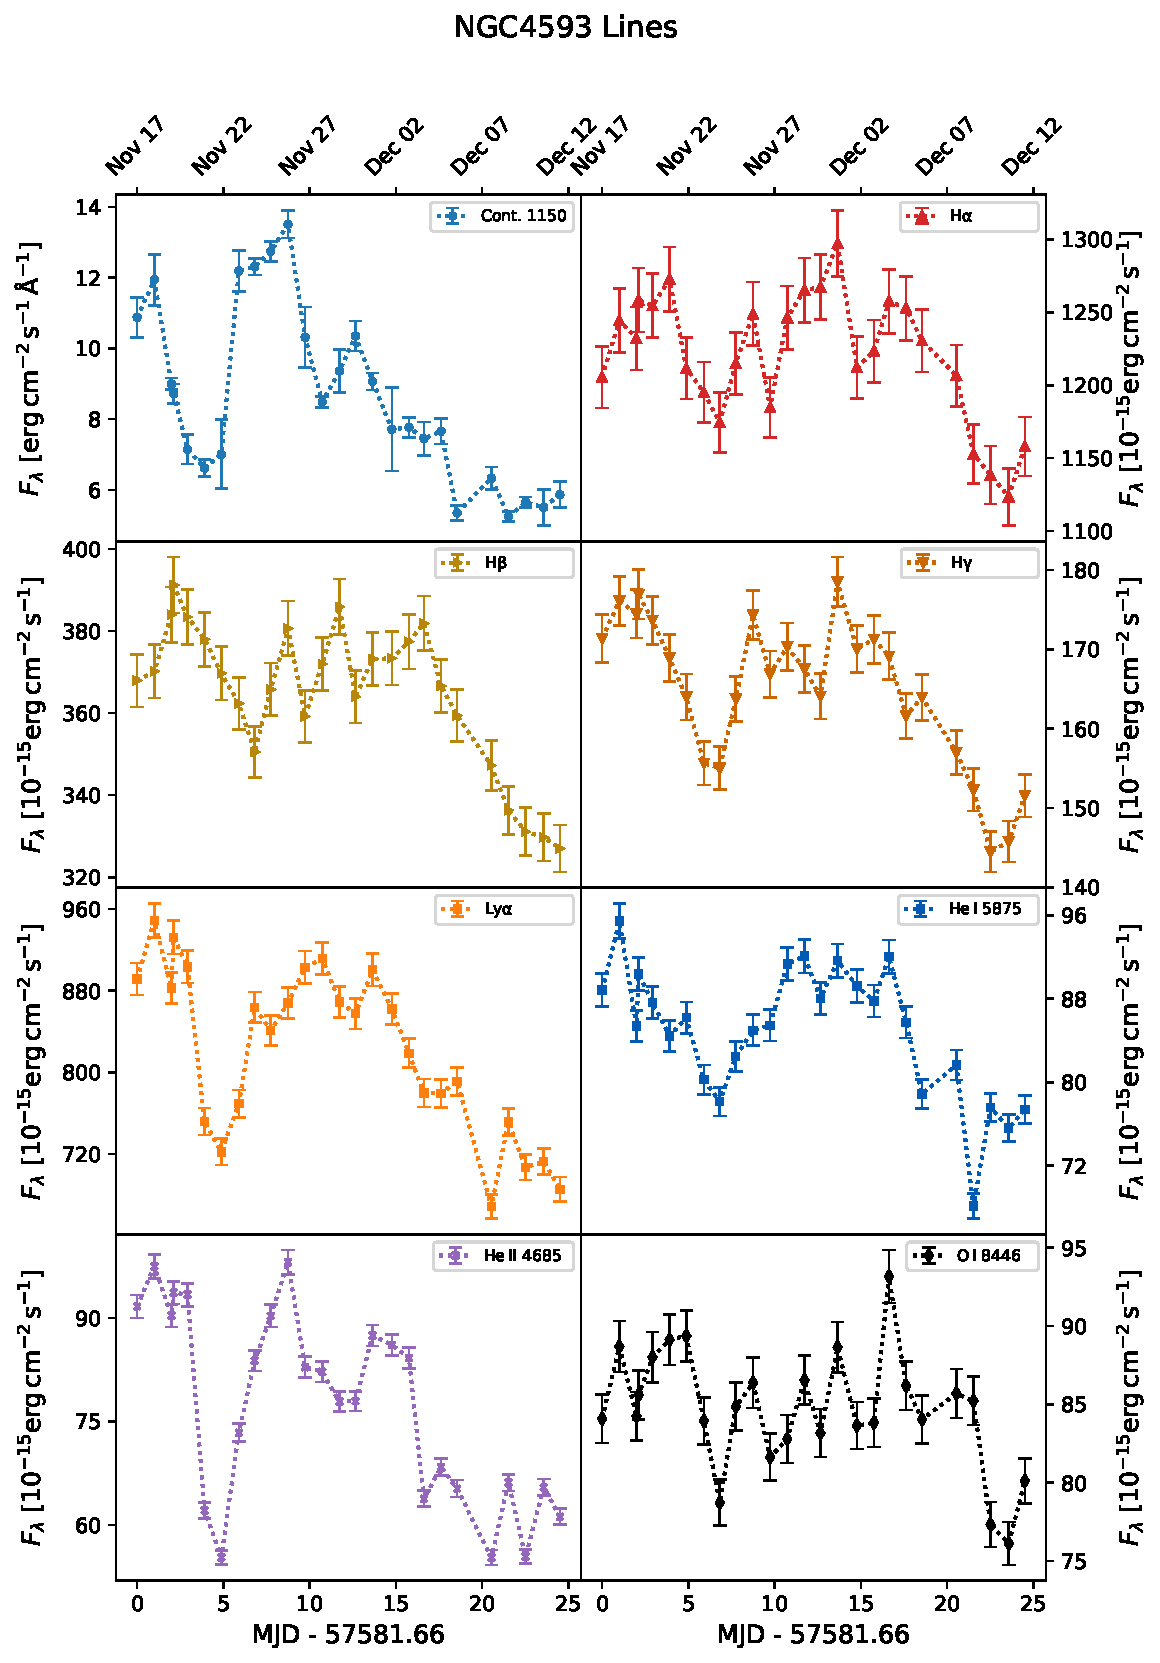
\includegraphics[width=0.9\textwidth]{pictures/Chapter4/lightcurves/NGC4593_Lines.pdf}
	\caption{AVG RMS Spektrum}
	\label{fig:emission_line_lightcurves}
\end{figure}

\section{Line Profiles}

\begin{figure}[!ht]
	\centering
	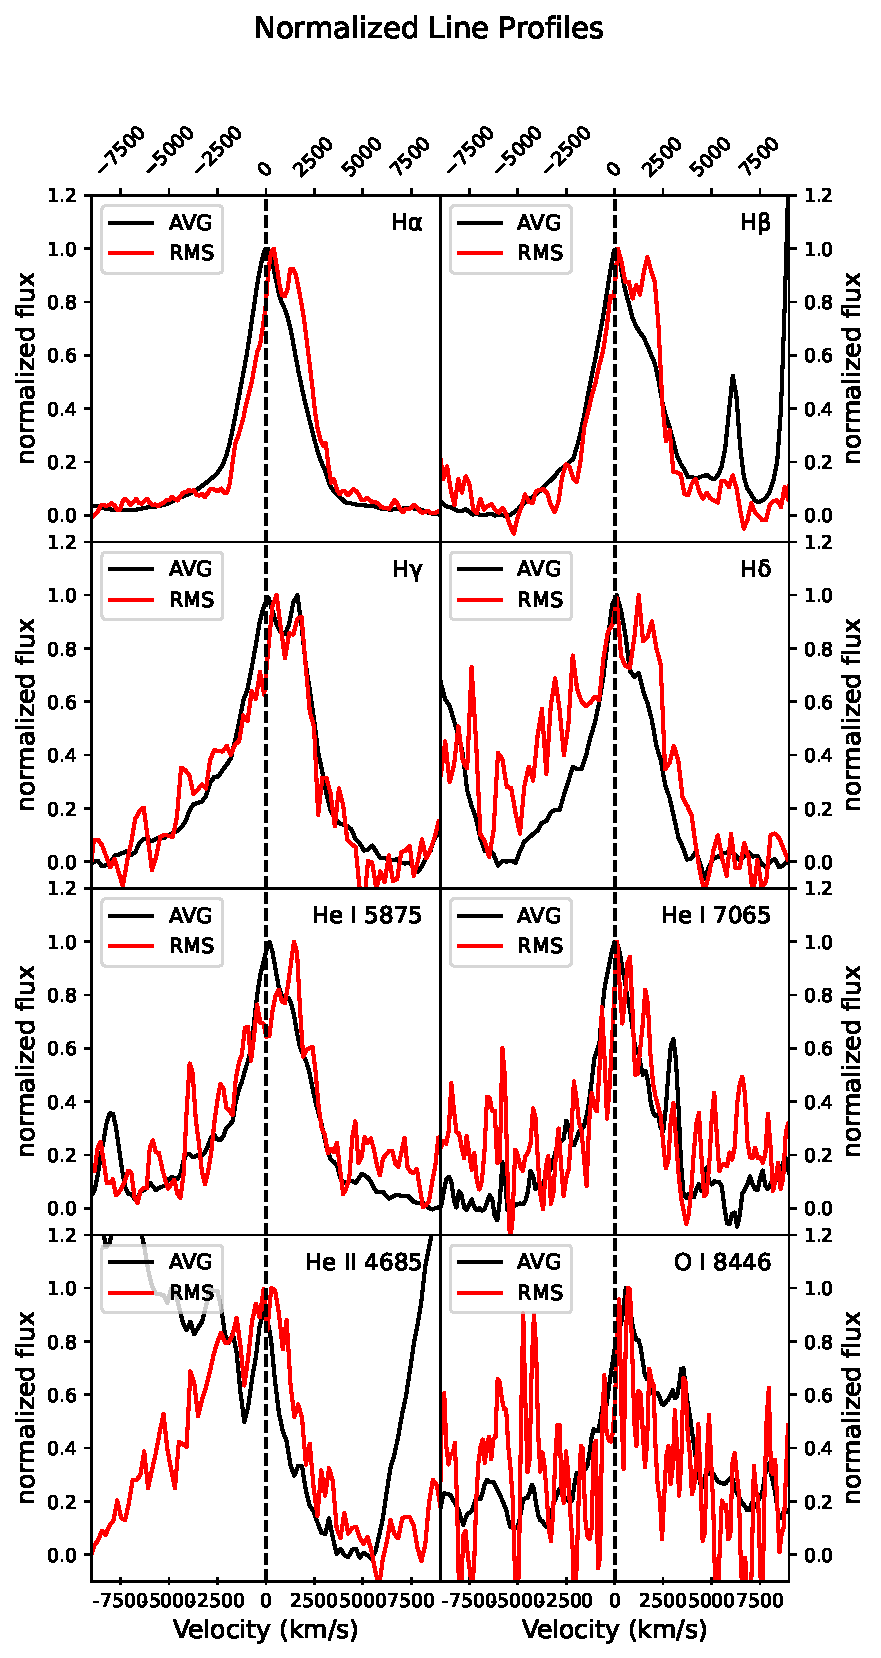
\includegraphics[width=0.9\textwidth]{pictures/Chapter4/line_profiles/Normalized_Line_Profiles.pdf}
	\caption{AVG RMS Spektrum}
	\label{fig:line_profiles}
\end{figure}

\section{Time Lag and BH Masses}

\begin{figure}[!ht]
	\centering
	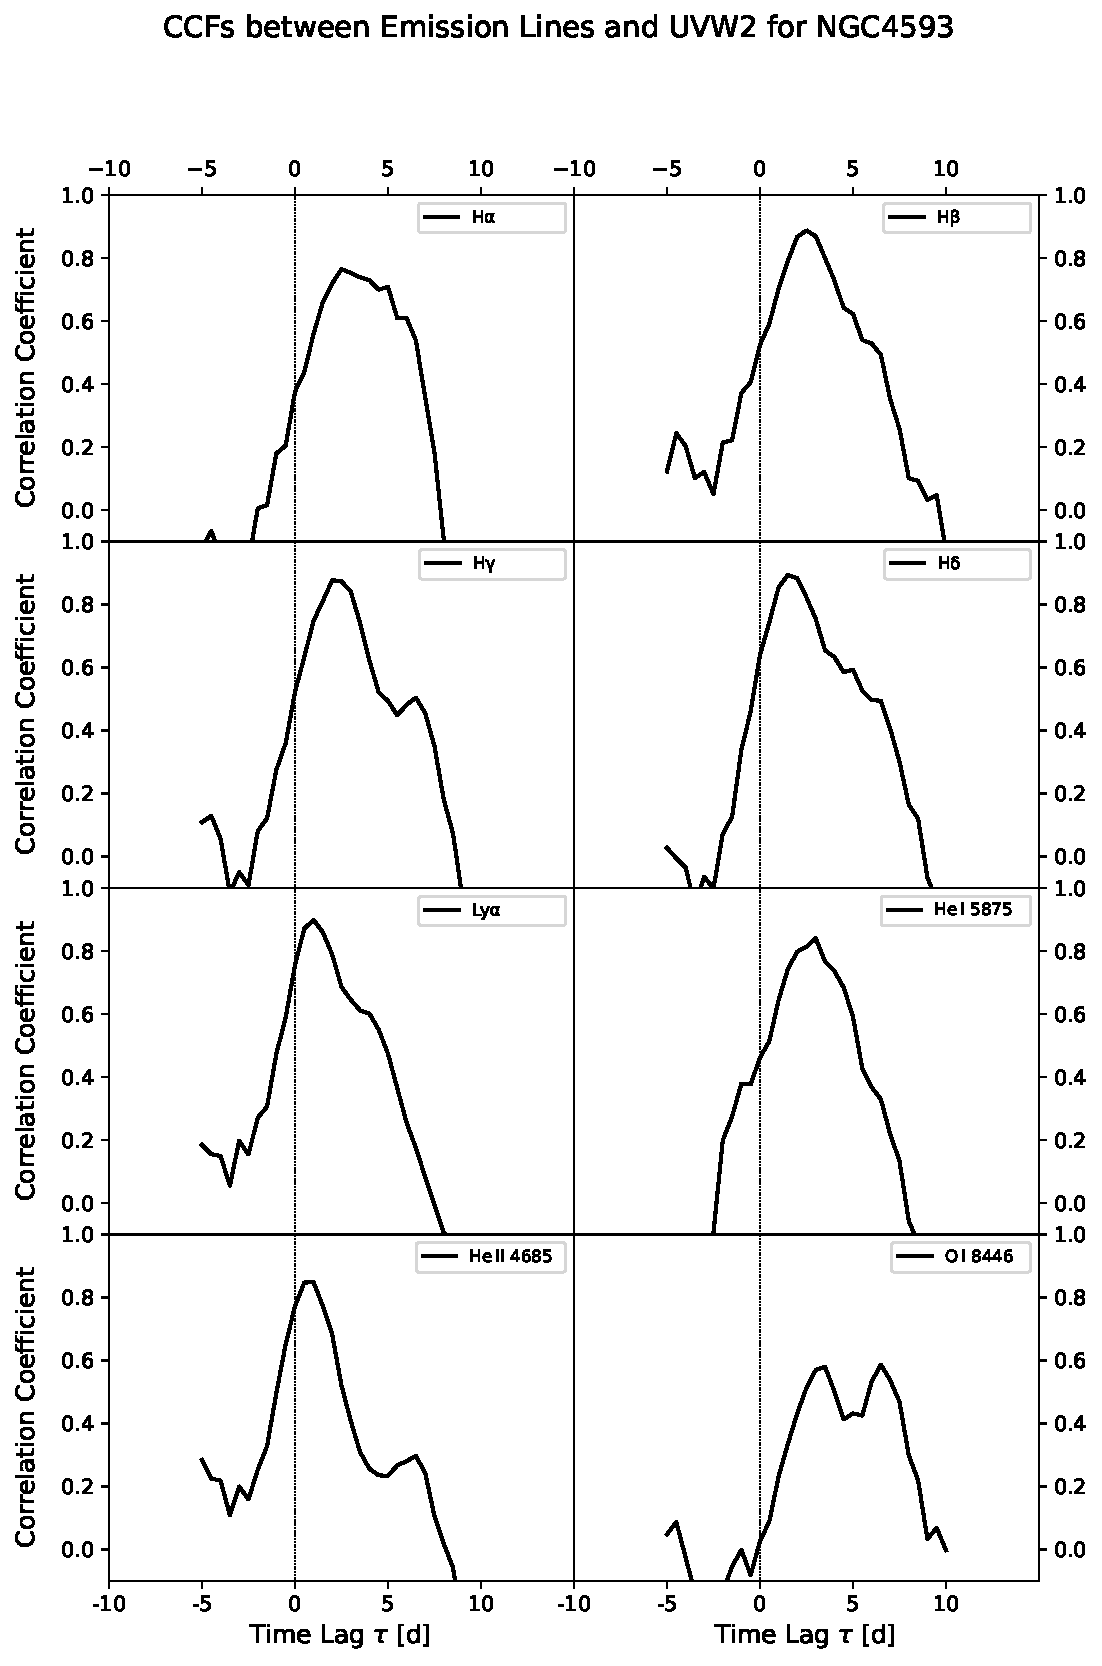
\includegraphics[width=0.9\textwidth]{pictures/Chapter4/ccfs/CCFs_H_He_LyA_O_UVW2.pdf}
	\caption{AVG RMS Spektrum}
	\label{fig:ccfs}
\end{figure}

\begin{figure}[!ht]
	\centering
	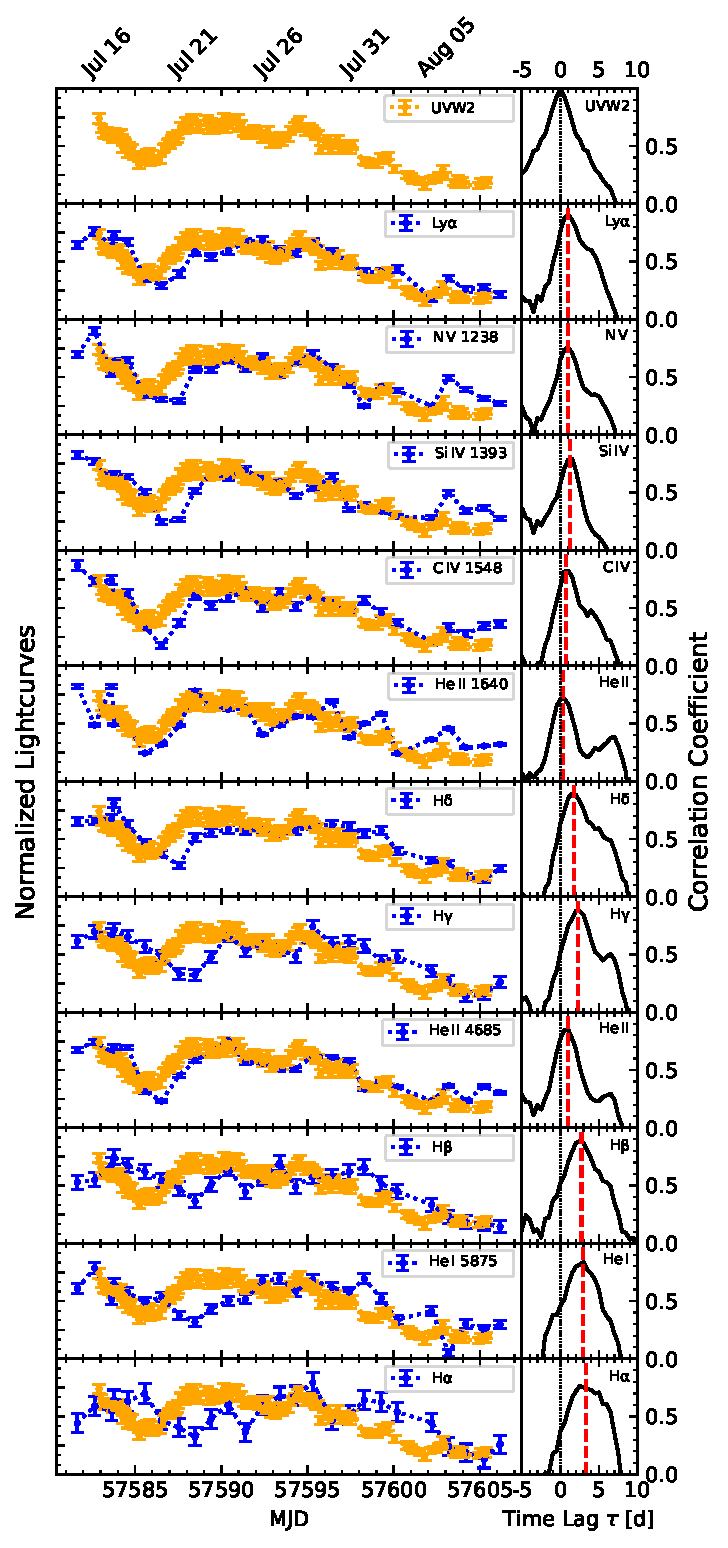
\includegraphics[width=0.7\textwidth]{pictures/Chapter4/lighcurves_and_ccfs_and_time_lag_tables/UV_to_HAlpha_ccfs_and_reference_lightcurves.pdf}
	\caption{AVG RMS Spektrum}
	\label{fig:ccfs_lightcurves}
\end{figure}

\section{Bowen Fluorescence}